\chapter{Datasets}
\label{sec:datasets}
In this chapter, the definition of experimental datasets is presented. These datasets exhibit various characteristics that our models aim to capture. The following sections provide a general overview of the source, size, and other elements that require consideration.
Three distinct datasets related to the energy domain, particularly in the context of time series data, were considered for our experiments. The primary focus, especially for the univariate approaches outlined in section \ref{sec: uni and multi}, was a form of 'power delivered.' For the multivariate approaches, additional features were also considered, if available, and virtual features were established, such as a daily sine or cosine.
All three datasets are open-source, and this section will describe the original state of the datasets. Additionally, details about how feature columns were added, excluded, or transformed will be discussed.
\subsection*{London Smart Meter dataset}
\label{subsec:LSM}
The London Smart Meter Dataset \cite{LSMsource} contains energy consumption readings for a set of 5,567 London Households that took part in the UK Power Networks led Low Carbon London project between November 2011 and February 2014.
Readings were taken at half hourly intervals. The customers in the trial were recruited as a balanced sample representative of the Greater London population.
The dataset contains energy consumption, in kWh (per half hour), unique household identifier, date and time. No further feature extraction steps were performed. Only the virtual samples described in section \ref{sec: uni and multi} were added. Moreover, the unique IDs, as previously mentioned, were utilized as categorical conditions, while weekly/yearly sine and cosine values served as continual conditions for our entity embedding, as described in section \ref{sec:unet time series}.
An overview of all parameters can be seen in table \ref{table:lsm params}. In figure \ref{fig:one_year_lsm} a year of a randomly picked household is shown. One year is depicted for a randomly sampled household and also a rolling mean of one week (336 timestamps).\newline
\begin{figure}
    \centering
    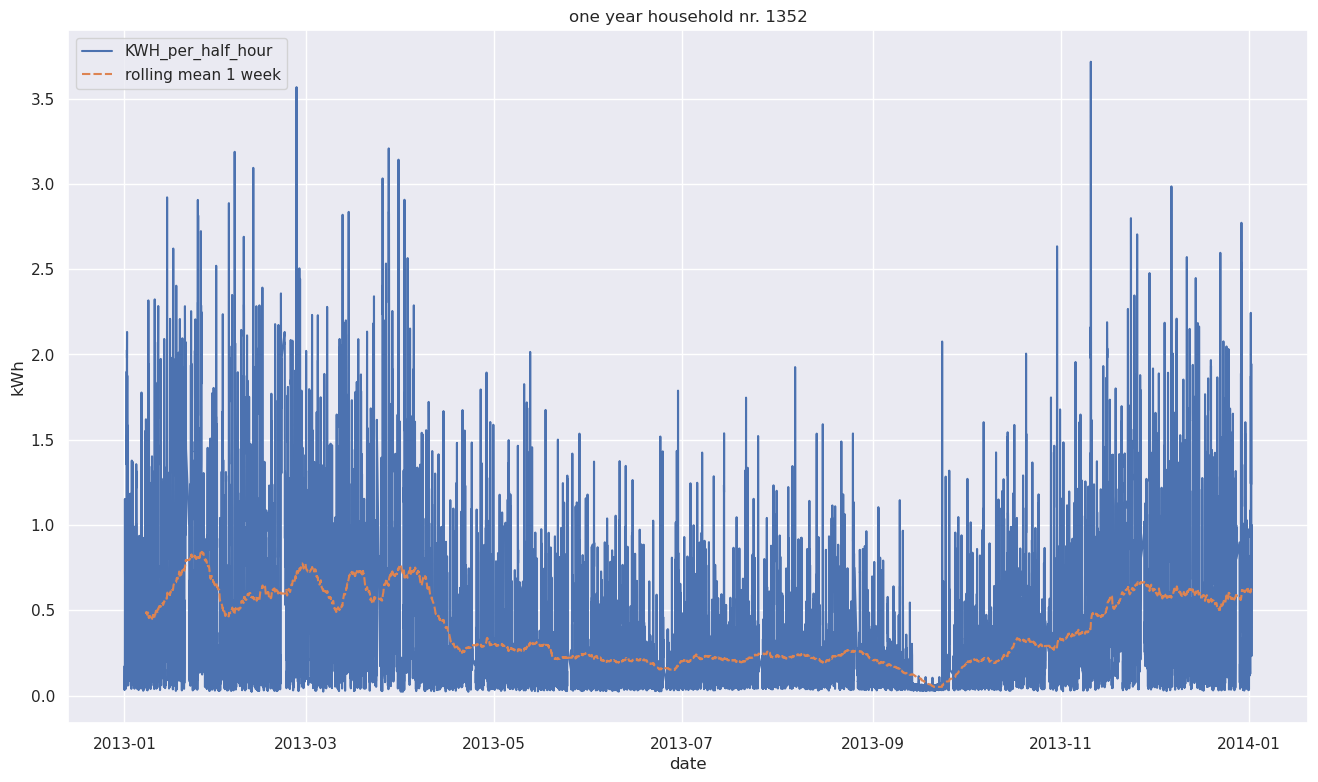
\includegraphics[width = \textwidth]{images/one_year_rm_lsm1357.png}
    \caption{Power consumption of a randomly picked LSM household for one year and a rolling mean for one week.}
    \label{fig:one_year_lsm}
\end{figure}
\begin{table}[h!]
    \centering
    \begin{tabular}{|c c c c c c|} 
         \hline
         name & dtype & type & univariate & multivariate & augmentation\\ [0.5ex] 
         \hline\hline
         kWperhalfhour & float & time series & \checkmark & \checkmark & normalized\\ 
         \hline
         daily sine & float & time series & - & \checkmark & -\\ 
         \hline
         daily cosine & float & time series & - & \checkmark & -\\ 
         \hline
         weekly sine & float & continual & \checkmark & \checkmark & - \\ 
         \hline
         weekly cosine & float & continual & \checkmark & \checkmark & -\\ 
         \hline
         yearly sine & float & continual & \checkmark & \checkmark & -\\ 
         \hline
         yearly cosine & float & continual & \checkmark & \checkmark & -\\ 
         \hline
         household ID & string & categorical & \checkmark & \checkmark & label encoded\\ 
         \hline
        \end{tabular}
    \caption{Overview of different targets and conditional data used for London Smart Meter Experiments.}
    \label{table:lsm params}
\end{table}

\subsection*{OpenMeter dataset} 
\label{subsec:openemter}
Open Meter \cite{OMsource} is a open platform where people, communes or institutions provide data about their power usage. This power is measured in watt in a 15-min resolution.
Providers also leave information about the usage, how much area their household or business occupies and location information to narrow down geographical context in Germany.
Open Meter also provides weather data for almost all sensors which can also be added to the training. During experiments categorical conditions city and post code are taken into consideration as well as area, weekly/yearly sine and weekly/yearly cosine for continual conditions. We also added the daily sine, daily cosine and temperature as targets for the multivariate approach.
An overview of all parameters can be seen in table \ref{table:openmeter params}.\newline
\begin{figure}[!h]
    \centering
    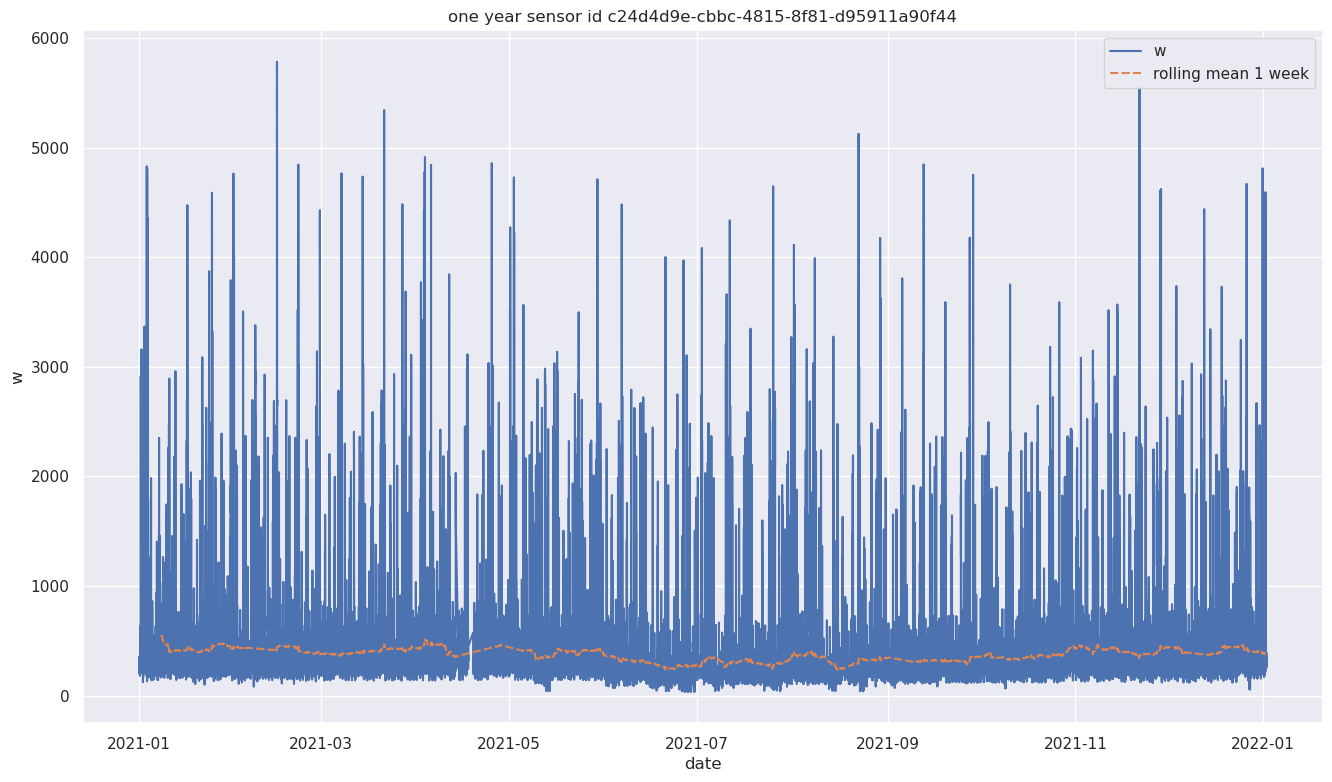
\includegraphics[width = \textwidth]{images/one_year_rolling_mean_om.png}
    \caption{Power consumption of a randomly picked OpenMeter sensor for one year and a rolling mean for one week.}
    \label{fig:one_year_lsm}
\end{figure}
\begin{table}[!h]
    \centering
    \begin{tabular}{|c c c c c c|}
         \hline
         name & dtype & type & univariate & multivariate & augmentation\\ [0.5ex] 
         \hline\hline
         power used & float & time series & \checkmark & \checkmark & normalized\\ 
         \hline
         temperature & float & time series & - & \checkmark & normalized\\ 
         \hline
         daily sine & float & time series & - & \checkmark & -\\ 
         \hline
         daily cosine & float & time series & - & \checkmark & -\\ 
         \hline
         weekly sine & float & continual & \checkmark & \checkmark & -\\ 
         \hline
         weekly cosine & float & continual & \checkmark & \checkmark & -\\ 
         \hline
         yearly sine & float & continual & \checkmark & \checkmark & -\\ 
         \hline
         yearly cosine & float & continual & \checkmark & \checkmark & -\\ 
         \hline
         area & float & continual & \checkmark & \checkmark & label encoded\\ 
         \hline
         city & string & categorical & \checkmark & \checkmark & label encoded\\ 
         \hline
         post code & string & categorical & \checkmark & \checkmark & label encoded\\ 
         \hline
        \end{tabular}
    \caption{Overview of different targets and conditional data used for Open Meter Experiments.}
    \label{table:openmeter params}
\end{table}
\newpage
\subsection*{ACN dataset}
\label{subsec:ACN}
The Adaptive Charging Network (ACN) Dataset \cite{ACNsource} provides information about electrical vehicle (EV) charging sessions. Gathered at different sites (caltech, jpl and office) that contain multiple charging stations.
The original dataset contained mostly technical information about the power delivery and time of occupation. The data was expanded by incorporating weather information, such as temperature and humidity. Also some feature crafting was performed to 
create fields like chargingTime, parkingTime and idleTime. All fields considered can be seen in table \ref{table:acn params}.
\begin{table}[h!]
    \centering
    \begin{tabular}{|c c c c|} 
         \hline
         name & dtype & type  & augmentation\\ [0.5ex] 
         \hline\hline
         kWhDelivered & float & time series  & normalized\\ 
         \hline
         chargingTime & float & time series  & normalized\\ 
         \hline
         idleTime & float & time series   & normalized\\ 
         \hline
         Temperature & float & time series   & normalized\\ 
         \hline
         2 metre relative humidity & float & time series   & normalized\\ 
         \hline
         2 metre specific humidity & float & time series   & normalized\\ 
         \hline
         weekly sine & float & continual   & -\\ 
         \hline
         weekly cosine & float & continual   & -\\ 
         \hline
         yearly sine & float & continual   & -\\ 
         \hline
         yearly cosine & float & continual   & -\\ 
         \hline
         siteType & float & categorical   & label encoded\\ 
         \hline
        \end{tabular}
    \caption{Overview of different targets and conditional data used for ACN Experiments.}
    \label{table:acn params}
\end{table}
For the ACN dataset we decided to directly synthesize multivariate data so there won't be a distinction during evaluation.
The final dataset we used was derived from combining the ACN caltech site dataset with the ACN jpl site dataset. 
\begin{figure}[h!]
    \centering
    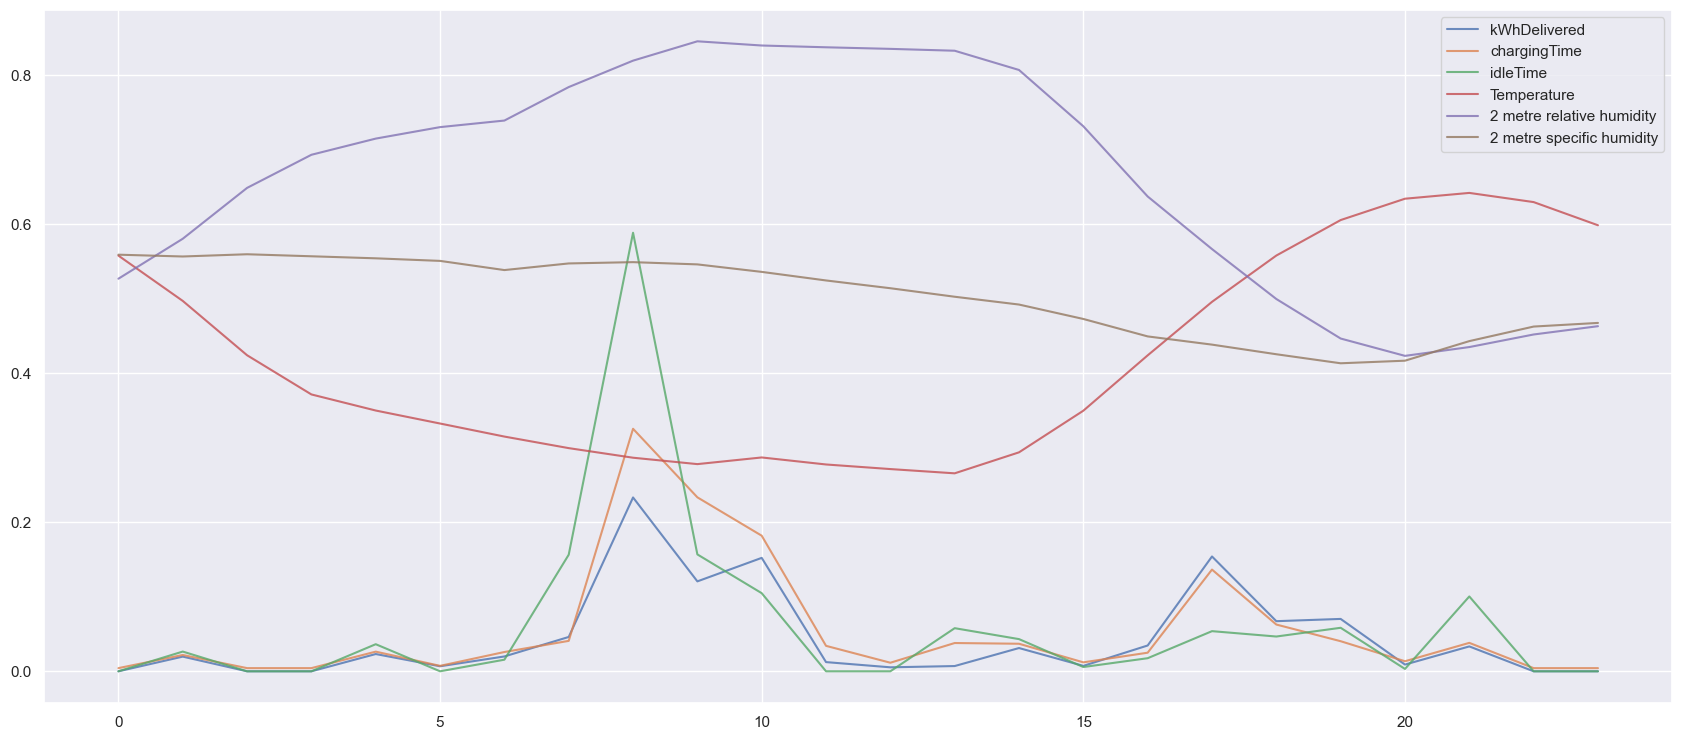
\includegraphics[width=\textwidth]{images/acn_sample.png}
    \caption{A multivariate sample from the ACN dataset.}
    \label{fig:ACN sample}
\end{figure}